\section{Mediciones}

Como sabemos el código corre en un tiempo $O(n log n)$ pero para poder demostrar que el código en realidad demora dicho tiempo, vamos a estar realizando una medición sobre el algoritmo. 

El método de medición consiste en realizar un set de datos usando un código que genera una cantidad de datos igual al parámetro de entrada, es decir, si el parámetro de entrada es 10, va a generar un archivo \textit{10.txt} con 10 rivales. Si se pasa una lista de M valores, genera M archivo con dichos valores (el parámetro esta hardcodeado en el archivo python).

Luego, corremos el código en modo de medición usando el comando python tp1.py --medir (tener cuidado con el -- de latex, puede fallar al copiarlo directamente), el cual realiza la medición de los tiempos por cada uno de los archivos generados anteriormente y guarda el resultada en un archivo llamado \textit{mediciones.txt} con el siguiente formato: 

\begin{figure}[H]
\centering
\begin{lstlisting}[style=fileformat]
10,tiempo de n=10
100,tiempo de n=100
1000,tiempo de n=1000
....
N,tiempo de n=N
\end{lstlisting}
\label{cod:fileOrdenamiento}
\caption{Archivo mediciones.txt}
\end{figure}

en donde, cada fila indica el tiempo que demoro el algoritmo con la cantidad de N datos en el archivo. De esta forma vamos a poder graficar los resultados y aproximar dicho puntos usando el método de cuadrado mínimo.

La siguiente figura muestra la aproximacion de las funciones $O(n log n)$ y $O(n^2)$ viendo que los puntos se aproximan mejor a una función de $O(n log n)$ que al tiempo de $O(n^2)$, demostrando que la teoria es correcta. 

\begin{figure}[H]
    \centering
    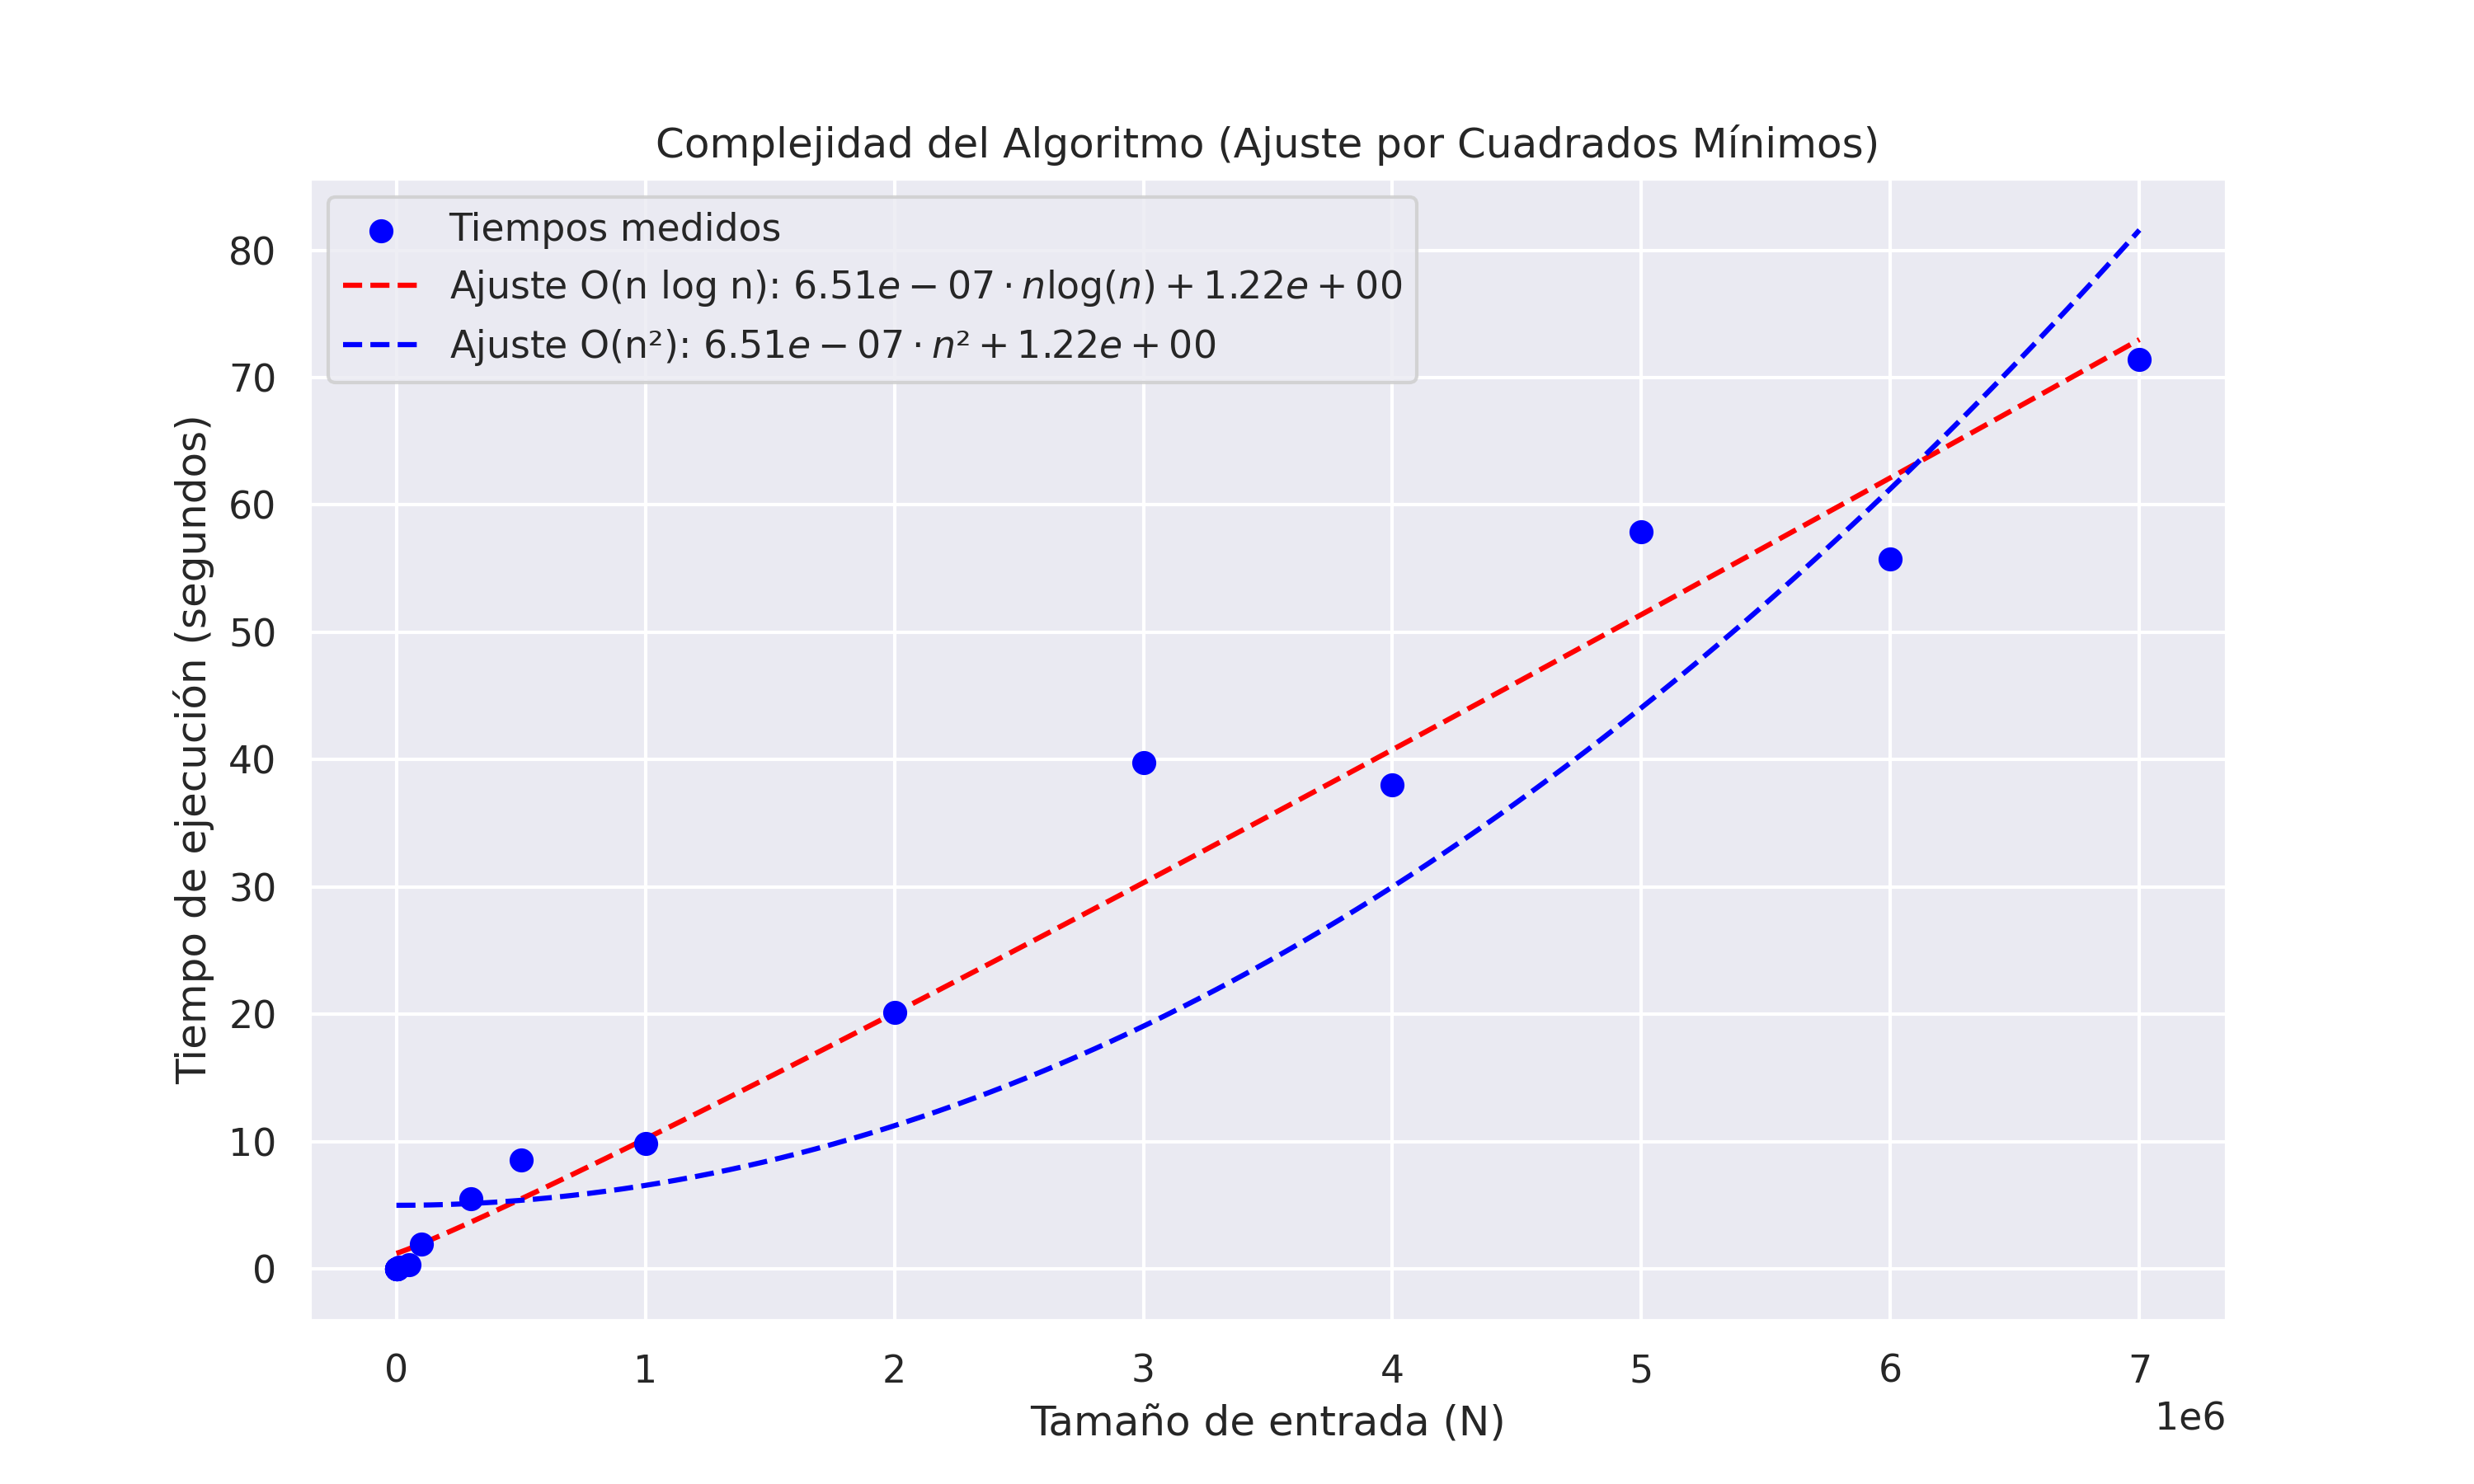
\includegraphics[width=1\textwidth]{img/tiempos.png}
\end{figure}

Es importante mostrar el error de la función aproximada con el teórico de esta forma podemos demostrar de una forma mas teórica a que función corresponde mas, demostrando que de forma teórica el error de la aproximación de $O(n log n)$  es menor al error de $O(n^2)$. Esto lo observamos en la siguiente figura.

\begin{figure}[H]
    \centering
    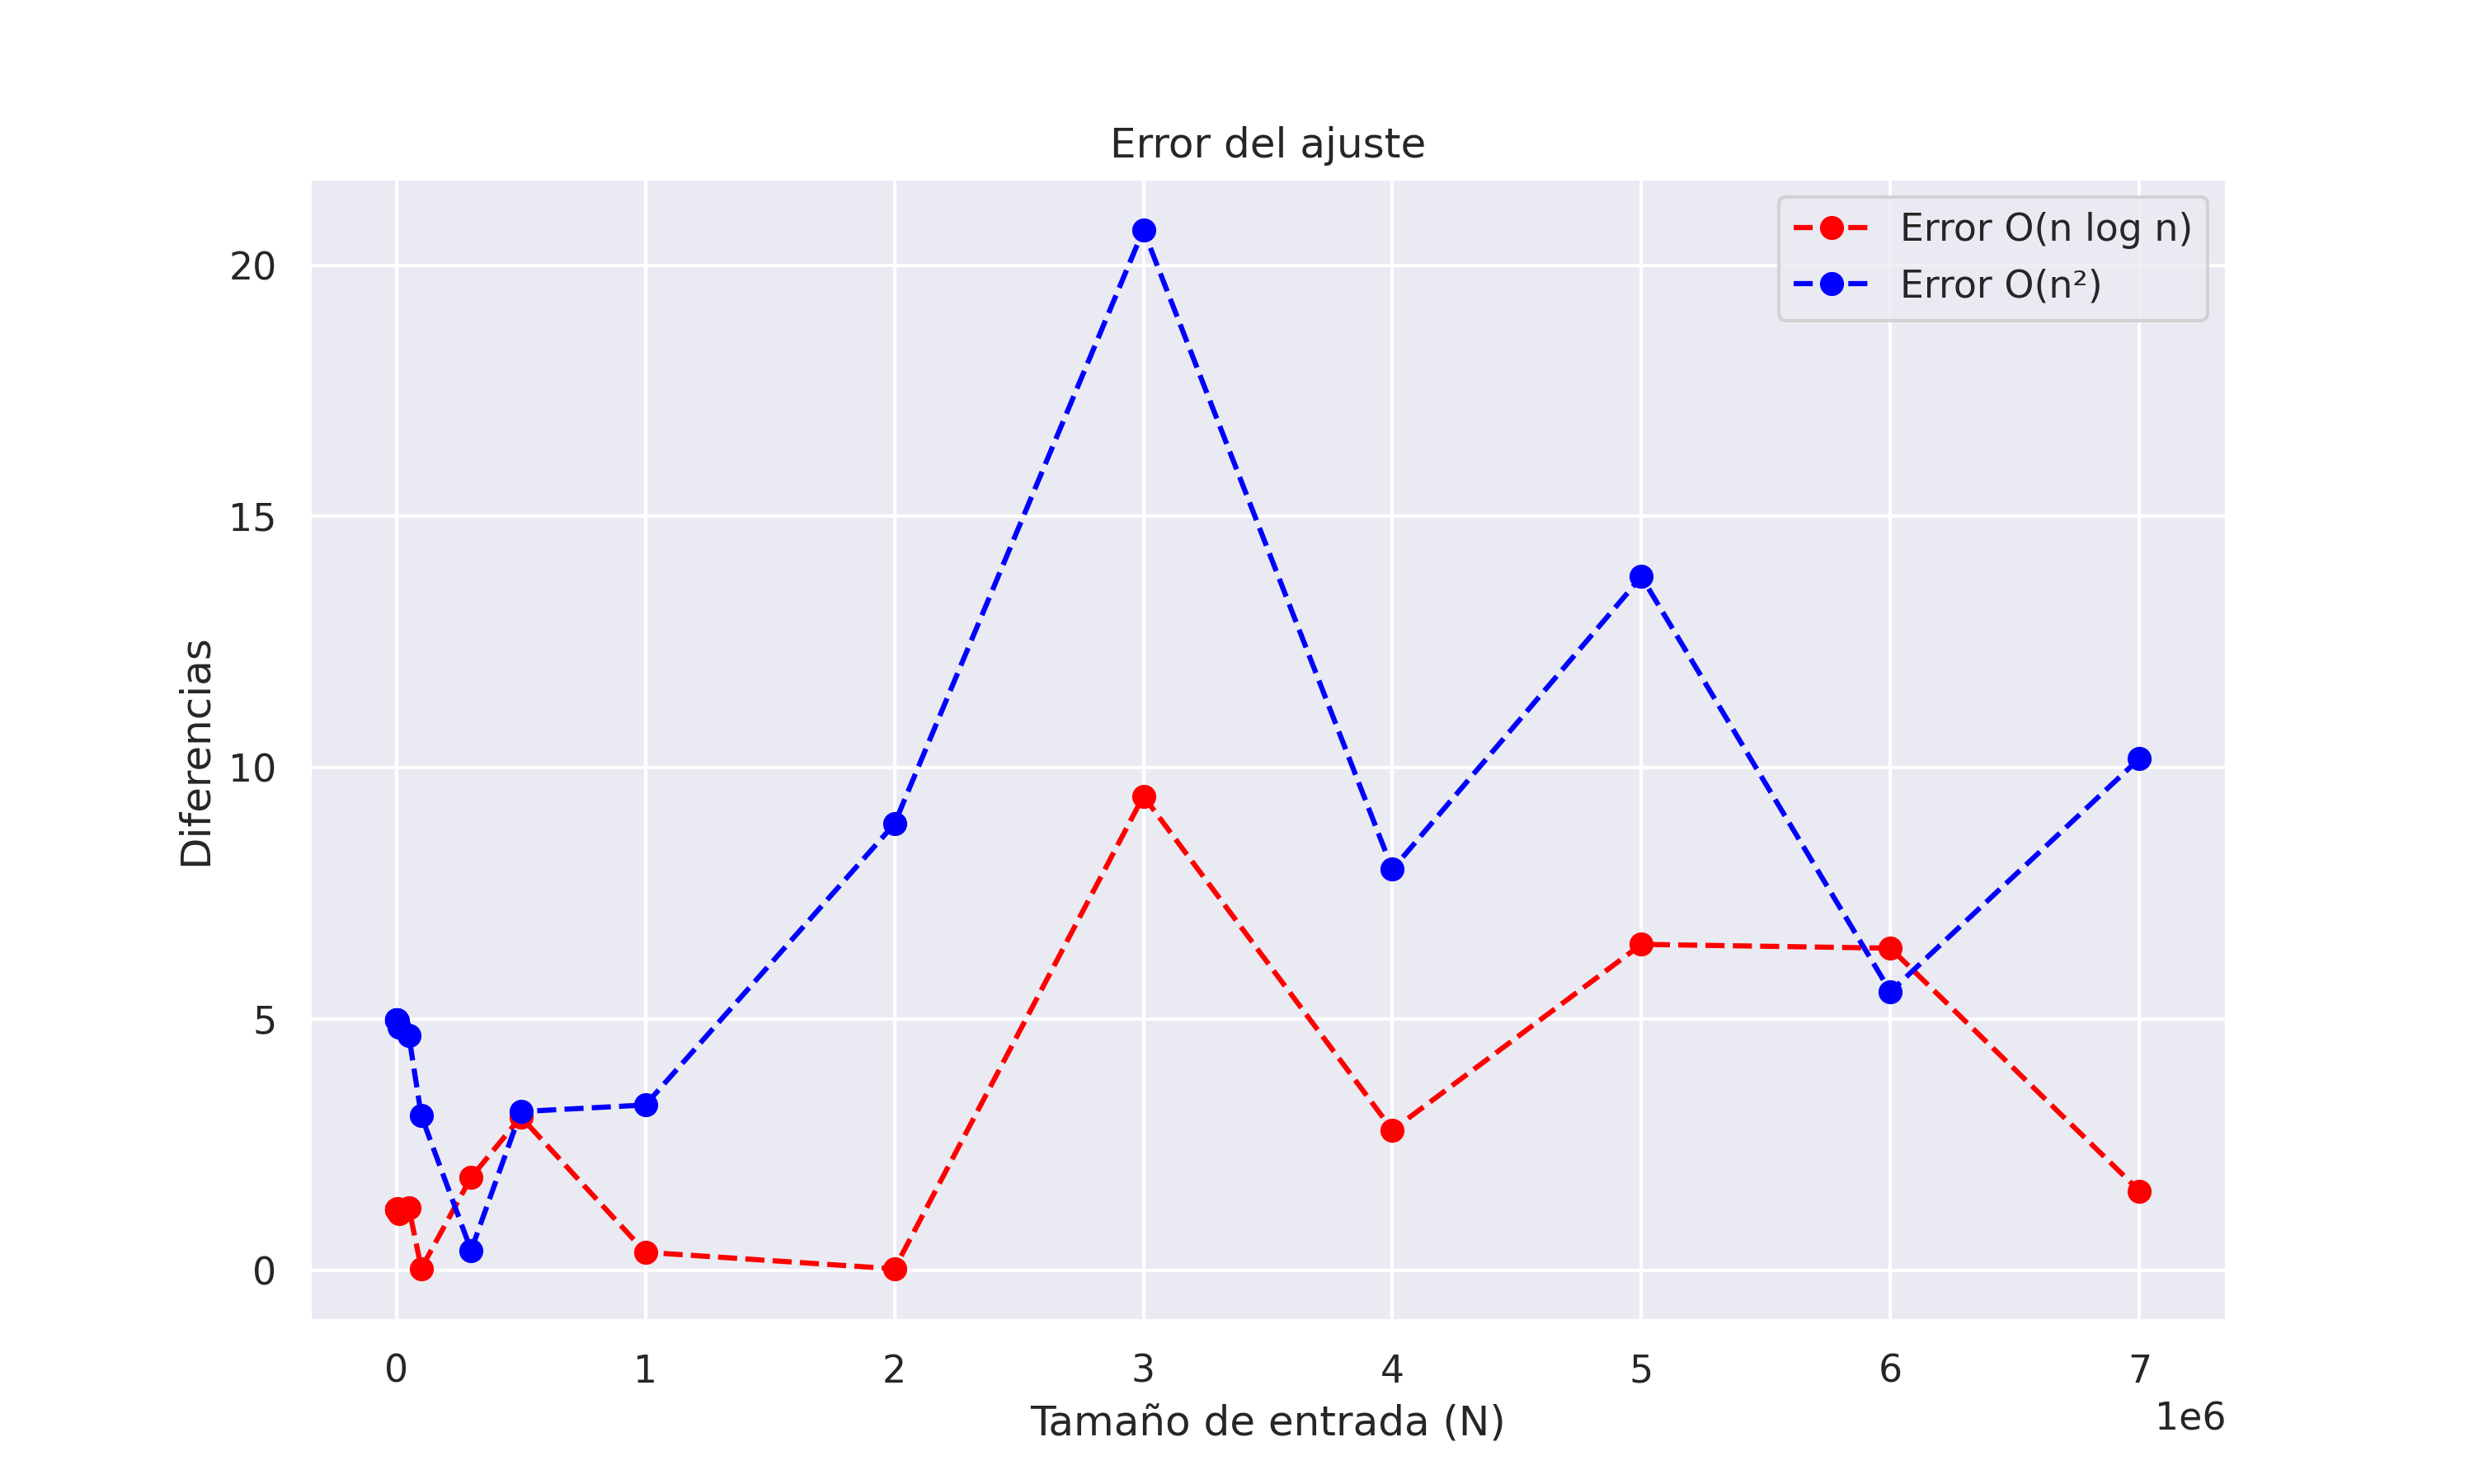
\includegraphics[width=1\textwidth]{img/error.png}
\end{figure}

notar, que en algunos datos el error de $O(n^2)$ es menor al de $O(nlogn)$, pero a nivel general, los datos se comporta mejor a la función de $O(nlogn)$.


Para obtener mas detalle de como correr los archivos y replicar el resultados, revisar el readme.md del repositorio.


